% This TeX document is part of the manual of the GNU Astronomy
% Utilities (Gnuastro). A Makefile is also distributed which allows
% you to compile this TeX file in the desired manner.
%
% Original author:
%     Mohammad Akhlaghi <mohammad@akhlaghi.org>
% Contributing author(s):
% Copyright (C) 2015-2020, Free Software Foundation, Inc.
%
% Gnuastro is free software: you can redistribute it and/or modify it
% under the terms of the GNU General Public License as published by
% the Free Software Foundation, either version 3 of the License, or
% (at your option) any later version.
%
% Gnuastro is distributed in the hope that it will be useful, but
% WITHOUT ANY WARRANTY; without even the implied warranty of
% MERCHANTABILITY or FITNESS FOR A PARTICULAR PURPOSE.  See the GNU
% General Public License for more details.
%
% You should have received a copy of the GNU General Public License
% along with Gnuastro. If not, see <http://www.gnu.org/licenses/>.

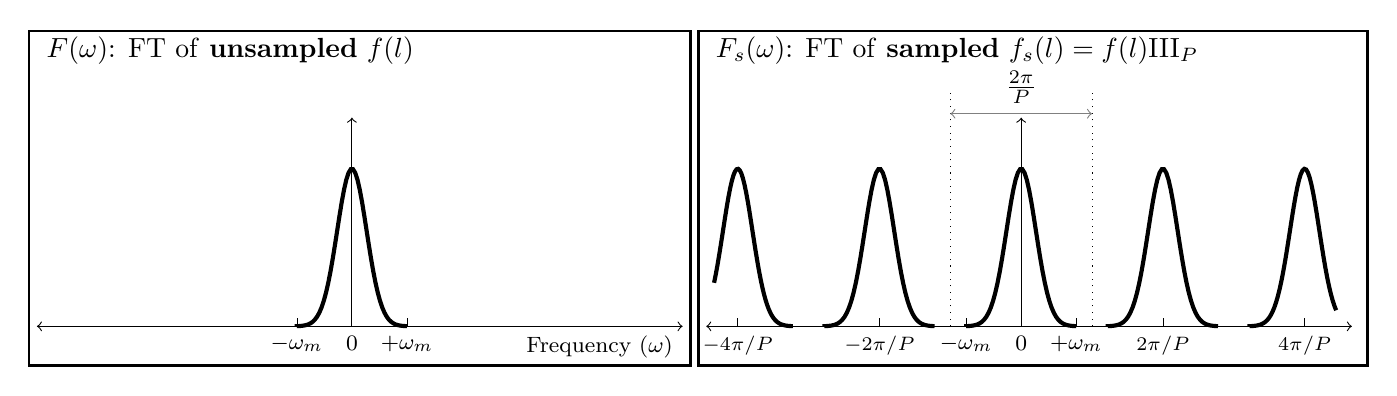
\begin{tikzpicture}[samples=50]

  %% Border rectangle and label.
  \draw [line width=1pt] (0,0) rectangle (8.4cm, 4.25cm);
  \draw [anchor=south west] (0.1cm, 3.7cm)
  node {$F(\omega)$: FT of \textbf{unsampled} $f(l)$};


  %% Draw the axis:
  \draw[<->] (0.1cm, 0.5cm) -- (8.3cm, 0.5cm);
  \draw[anchor=north east] (8.3cm, 0.5cm) node {\footnotesize Frequency ($\omega$)};
  \draw[->] (4.1cm, 0.5cm) -- (4.1cm, 3.15cm);


  %% Draw the main plot
  \draw[line width=1.5pt, domain=3.4:4.8]
  (3.4,0.5) -- plot (\x, {2*exp(-((\x-4.1)^2)/0.07)+0.5});
  \draw[very thin, anchor=north] (3.4,0.6) -- (3.4,0.5)
  node {\footnotesize $-\omega_m$};
  \draw[very thin, anchor=north] (4.8,0.6) -- (4.8,0.5)
  node {\footnotesize $+\omega_m$};
  \draw[anchor=north] (4.1,0.5) node {\footnotesize $0$};








  %% Border rectangle and label.
  \draw [line width=1pt] (8.5cm,0) rectangle (17cm, 4.25cm);
  \draw [anchor=south west] (8.6cm, 3.7cm)
  node {$F_s(\omega)$: FT of \textbf{sampled} $f_s(l)=f(l)\mathrm{III}_P$};


  %% Draw the axis:
  \draw[<->] (8.6cm, 0.5cm) -- (16.8cm, 0.5cm);
  \draw[->] (12.6cm, 0.5cm) -- (12.6cm, 3.15cm);


  %% Draw the main plot
  \draw[line width=1.5pt, domain=11.9:13.3]
  (11.9,0.5) -- plot (\x, {2*exp(-((\x-12.6)^2)/0.07)+0.5});
  \draw[very thin, anchor=north] (11.9,0.6) -- (11.9,0.5)
  node {\footnotesize $-\omega_m$};
  \draw[very thin, anchor=north] (13.3,0.6) -- (13.3,0.5)
  node {\footnotesize $+\omega_m$};
  \draw[anchor=north] (12.6,0.5) node {\footnotesize $0$};


  %% Draw the region:
  \draw[anchor=east, dotted] (11.7,0.5) -- (11.7,3.5);
  \draw[anchor=west, dotted] (13.5,0.5) -- (13.5,3.5);
  \draw[<->, color=gray, thin] (11.7,3.2) -- (13.5,3.2);
  \draw[anchor=south] (12.6,3.2) node {$\frac{2{\pi}}{P}$};


  %% Next plot (first positive)
  \draw[line width=1.5pt, domain=13.7:15.1]
  (13.7,0.5) -- plot (\x, {2*exp(-((\x-14.4)^2)/0.07)+0.5});
  \draw[very thin, anchor=north]
  (14.4,0.6) -- (14.4,0.5) node {\scriptsize $2{\pi}/P$};

  %% Next plot (second positive)
  \draw[line width=1.5pt, domain=15.5:16.6]
  (15.5,0.5) -- plot (\x, {2*exp(-((\x-16.2)^2)/0.07)+0.5});
  \draw[very thin, anchor=north]
  (16.2,0.6) -- (16.2,0.5) node {\scriptsize $4{\pi}/P$};

  %% Next plot (first negative)
  \draw[line width=1.5pt, domain=10.1:11.5]
  (10.1,0.5) -- plot (\x, {2*exp(-((\x-10.8)^2)/0.07)+0.5});
  \draw[very thin, anchor=north]
  (10.8,0.6) -- (10.8,0.5) node {\scriptsize $-2{\pi}/P$};

  %% Next plot (second negative)
  \draw[line width=1.5pt, domain=8.7:9.7]
  plot (\x, {2*exp(-((\x-9)^2)/0.07)+0.5});
  \draw[very thin, anchor=north]
  (9,0.6) -- (9,0.5) node {\scriptsize $-4{\pi}/P$};

\end{tikzpicture}
